
\tikzstyle{input_neuron}=[circle,draw=red!50,fill=orange!10,thick,minimum size=.2mm]
\tikzstyle{hidden_neuron}=[circle,draw=blue!50,fill=blue!10,thick,minimum size=1mm]
\tikzstyle{output_neuron}=[circle,draw=green!50,fill=green!20,thick,minimum size=1mm]
\tikzstyle{output}=[circle,draw=green!50,fill=green!20,thick,minimum size=1mm]
\tikzstyle{positive}=[circle,draw=red!50,fill=red!10,thick,minimum size=.2mm]
\tikzstyle{negative}=[circle,draw=blue!50,fill=blue!10,thick,minimum size=1mm]
\resizebox{6cm}{6cm}{%
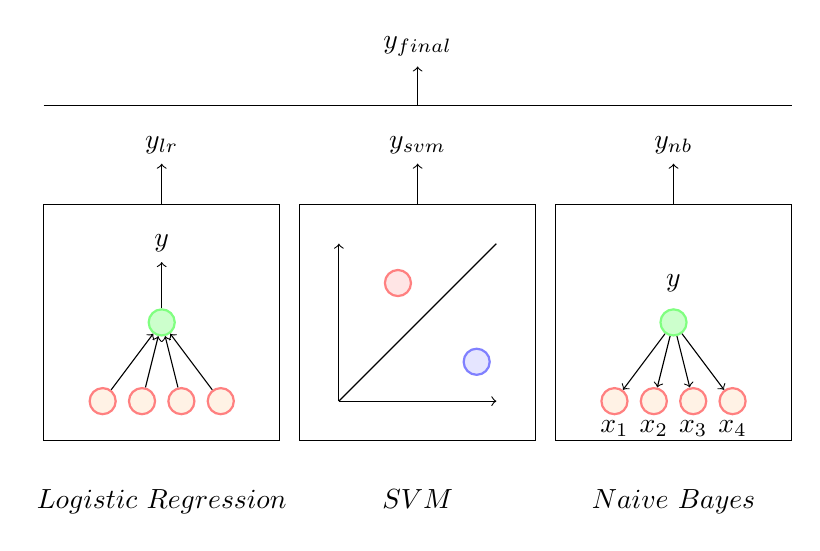
\begin{tikzpicture}
						
	\node [input_neuron] (in0) at (0.75,0.5) {};
	\node [input_neuron] (in1) at (1.25,0.5) {};
	\node [input_neuron] (in2) at (1.75,0.5) {} ;
	\node [input_neuron] (in3) at (2.25,0.5) {} ;
						
	\node [output_neuron] (out0) at (1.5,1.5)  {} ;
						
	\node (output0) at (1.5,2.5)  {$y$} ;
	\node (output1) at (1.5,3.75)  {$y_{lr}$} ;
	\draw (0,0) rectangle  (3,3);
	\draw [->] (in0) -- (out0);
	\draw [->] (in1) -- (out0);
	\draw [->] (in2) -- (out0);
	\draw [->] (in3) -- (out0);
	\draw [->] (out0) -- (output0);
	\draw [->] (1.5,3) -- (output1);
	\node [below] (head) at (1.5,-0.5)  {$Logistic$ $Regression$} ;
						
	\draw[->,xshift=0mm] (3.75,0.5) -- coordinate (x axis mid) (5.75,0.5);
	\draw[->,xshift=0mm] (3.75,0.5) -- coordinate (y axis mid)(3.75,2.5);
	\node [positive] (in0) at (4.5,2) {};
	\node [negative] (out0) at (5.5,1) {};
						
	\draw (3.25,0) rectangle  (6.25,3);
	\node (output2) at (4.75,3.75)  {$y_{svm}$} ;
	\draw [->] (4.75,3) -- (output2);
	\draw  (3.75,0.5) -- (5.75,2.5);
	\node [below] (head) at (4.75,-0.5)  {$SVM$} ;
						
	\draw (6.5,0) rectangle (9.5,3);
	\node (output3) at (8,3.75)  {$y_{nb}$} ;
	\draw [->] (8,3) -- (output3);
						
	\node [input_neuron] (in10) at (7.25,0.5) {};
	\node [input_neuron] (in11) at (7.75,0.5) {};
	\node [input_neuron] (in12) at (8.25,0.5) {} ;
	\node [input_neuron] (in13) at (8.75,0.5) {} ;
	\node at (7.25,0.15) {$x_1$};
	\node at (7.75,0.15) {$x_2$};
	\node at (8.25,0.15) {$x_3$};
	\node at (8.75,0.15) {$x_4$};
	\node [output_neuron] (out10) at (8,1.5)  {} ;
	\node (output0) at (8,2)  {$y$} ;
	\draw [->] (out10) -- (in10);
	\draw [->] (out10) -- (in11);
	\draw [->] (out10) -- (in12);
	\draw [->] (out10) -- (in13);
	\node [below] (head) at (8,-0.5)  {$Naive$ $Bayes$} ;
	\node (output3) at (4.75,5)  {$y_{final}$} ;
	\draw (0,4.25) -- (9.5,4.25);
	\draw [->] (4.75,4.25) -- (4.75,4.75);
\end{tikzpicture}
}